% to turn into handout mode, add [10pt, a4paper, handout]
\documentclass[10pt,a4paper, handout]{beamer}
\usepackage[latin1]{inputenc}
\usepackage{amsmath}
\usepackage{amsfonts}
\usepackage{amssymb}
\usepackage{graphicx}
\usetheme{Madrid}
\usepackage{ulem}
\usepackage{algorithm2e}
\usepackage{algpseudocode}
\usepackage{diffcoeff}
\usepackage{xcolor}
\usepackage{tikz}
\usepackage{cancel}
\usepackage{pgfplots}
\usepackage{background}
\usepackage{stmaryrd}
\usepackage{ulem}
\DeclareMathOperator*{\argmin}{\arg\!\min}



\algnewcommand\algorithmicinput{\textbf{Input:}}
\algnewcommand\Input{\item[\algorithmicinput]}

\algnewcommand\algorithmicoutput{\textbf{Output:}}
\algnewcommand\Output{\item[\algorithmicoutput]}

\algnewcommand\algorithmiceffect{\textbf{Effect:}}
\algnewcommand\Effect{\item[\algorithmiceffect]}


\newcommand{\biject}{\langle \cdot \rangle}
\newcommand{\bij}[1]{\langle {#1} \rangle}

\renewcommand{\S}{\mathcal{S}}
\newcommand{\A}{\mathcal{A}}
\newcommand{\R}{\mathcal{R}}
\renewcommand{\Pr}{\text{Pr}}
\DeclareMathOperator*{\argmax}{arg\,max}
\newcommand{\red}[1]{\textcolor{red}{#1}}
\newcommand{\iter}{\xrightarrow{I}}
\newcommand{\eval}{\xrightarrow{E}}
\newcommand{\bth}{{\boldsymbol{\theta}}}
\newcommand{\pth}{{\boldsymbol{\phi}}}
\renewcommand{\P}{\text{P}}
\newcommand{\Ex}{\mathbb{E}}
\newcommand{\iver}[1]{\llbracket  {#1} \rrbracket}


\newcommand{\bs}[1][]{%
	\begin{tikzpicture}[baseline,x=0.8\ht\strutbox,y=0.8\ht\strutbox,line width=0.125ex,#1]
		\def\arm{(-2.5,0.95) to (-2,0.95) (-1.9,1) to (-1.5,0) (-1.35,0) to (-0.8,0)};
		\draw \arm;
		\draw[xscale=-1] \arm;
		\def\headpart{(0.6,0) arc[start angle=-40, end angle=40,x radius=0.6,y radius=0.8]};
		\draw \headpart;
		\draw[xscale=-1] \headpart;
		\def\eye{(-0.075,0.15) .. controls (0.02,0) .. (0.075,-0.15)};
		\draw[shift={(-0.3,0.8)}] \eye;
		\draw[shift={(0,0.85)}] \eye;
		% draw mouth
		\draw (-0.1,0.2) to [out=15,in=-100] (0.4,0.95); 
\end{tikzpicture}}

%to disable pauses, uncomment
%\renewcommand{\onslide}[2]{#1}



\begin{document}

\title[Reinforcement Learning Basics Any\% Speedrun] %optional
{Reinforcement Learning Basics Any\% Speedrun }

 
\author[David Quarel] % (optional, for multiple authors)
{David Quarel}
 
\institute[ARENA] % (optional)
{
  ARENA
}
 
\date[8th June 2023] % (optional)
{Thursday, 8th June 2023}
 
\frame{\titlepage}

\begin{frame}
\frametitle{What is Reinforcement Learning?}
\begin{itemize}
	\item Up to this point we've been mostly within the regime of 
	supervised learning: Given some labelled data, train a model to
	minimise loss, then deploy to classify new data.
	\begin{enumerate}
		\pause 
		\item We have access to labelled training data, and only deploy
		the agent after we get good performance. Agent only sees 
		``real world'' once it's already performing well
		\pause 
		\item Data is i.i.d between batches
		\pause 
		\item No planning required, future predictions don't depend on past
		predictions
		\pause
	\end{enumerate}  
	\item RL is vastly different: Agent takes actions in an interactive environment,
	receive scalar reward as feedback. This lends itself to several problems:
	\pause
	\begin{enumerate}
		\item  \textbf{Sparse reward:} Very little feedback during learning 
		\pause
		\item \textbf{Reward attribution:} Hard to tell which action
		was the one that caused the good reward
		\pause
		\item \textbf{No ground truth} Optimal or even good policies
		may be unknown, (in pure RL settings) no data from good players to compare against
		\pause
		\item \textbf{Explore vs. Exploit tradeoff}: 
		\begin{enumerate}
			\item \textbf{Exploration:} Taking actions to learn how the 
			world works (and improve the policy).
			\item \textbf{Exploitation:} Taking actions that maximise the expected sum of reward given current policy.
		\end{enumerate}
	\pause 
	\item \textbf{Online only:} No clear distinction between training and testing.
	Agent gets dumped in the environment and must learn on the fly. 
	\end{enumerate} 
\end{itemize}
	
\end{frame}

 
\begin{frame}
\begin{figure}
	\centering
	\includegraphics[width=1\linewidth]{img/yann}
\end{figure}
\end{frame}
%
\begin{frame}
	\begin{figure}
	\includegraphics[width=1\linewidth]{img/cherry}
	\end{figure}
\end{frame}


\begin{frame}
	\frametitle{Multi-Armed Bandits}
	\begin{itemize}
		\item The simplest type of RL environment with interaction: (equivalent to
		MDP with 1-state)
		\pause
		\item Agent has a set of ``arms'' 
		(actions) $\A$. Environment has a family of reward distributions
		$\{p_a\}_{a \in \A}$ for each action.
		\pause
		\item On timestep $t$, agent chooses action $a_t$ and receives
		reward $r_t \sim p_{a_t}(\cdot)$. Distributions $p_i$ are unknown to agent.
		\pause
		\item Want to always choose the arm with the highest
		expected payout:
		$$
		q_*(a) = \mathbb{E}[r_t | a_t = a]
		$$
		\pause
		\item Need to balance trying all the arms to get a
		good estimate of the value of each arm, v.s. always trying
		to pull the best arm.
	\end{itemize}
\end{frame}

\begin{frame}
	\begin{figure}
		\centering
		\includegraphics[width=0.9\linewidth]{img/bandito}
		\label{fig:bandito}
	\end{figure}
\end{frame}

\begin{frame}{Bandito Algorithm}
	\begin{itemize}
		\item Keep track of $\hat{Q}(a)$, the estimated value of each arm
		after $t$ arm-pulls
		$$
		\hat{Q}_t(a) = \frac{\text{sum of rewards when $a$ taken up to $t$}}
		{\text{number of times $a$ taken prior to $t$}}
		= \frac{\sum_{i=1, a_i=a}^{t-1} r_t  }{\sum_{i=1,a_i=a}^{t-1} 1} 
		$$
		\pause 
		\item
		$\hat{Q}_t(a)$ represents the empirical average reward obtained from arm $a$
		up to time $t$. 
		\pause 
		\item In practice, easier to init 
		$\hat{Q}_1(a) = \hat{R}_1(a) = \hat{N}_1(a) = 0$ and
		\begin{align*}
			&\hat{R}_{t+1}(a) \leftarrow \hat{R}_{t}(a) + r_t \iver{a_t=a} 
		\quad \hat{N}_{t+1}(a) \leftarrow \hat{N}_{t}(a) + \iver{a_t=a} \\
		& \hat{Q}_{t+1}(a) \leftarrow \frac{\hat{R}_{t+1}(a)}{N_{t+1}(a)}
		\end{align*}
	where $\iver{P} = 1$ if $P$ evaluates to True, else $\iver{P}=0$.
	\pause 
	\item Choose arm with highest estimated payout: $a_t := \argmax \hat{Q}_t(a)$.
	\pause
	\item \textbf{Problem:} Can get stuck with a suboptimal arm.
	\end{itemize}
\end{frame}

\begin{frame}{Encouraging Exploration}
	\begin{enumerate}
		\item \textbf{First approach:} Just do random stuff every now and 
		again, hope for the best
		$$
		a^{\epsilon-greedy}_t = \begin{cases}
			\text{Do random action} & \text{Prob } \epsilon \\
			\argmax_{a'} Q_t(a') & \text{Prob } 1-\epsilon 
		\end{cases}
		$$
		\pause
		\item \textbf{Better approach:} Give a bonus to actions seldom taken
		$$
		a^{UCB}_t = \argmax_{a'}
		\left( 
		Q_t(a') + c \sqrt{\frac{\ln t}{N_t(a')}}
		\right)
		$$
		\pause
		\item \textbf{Intuition:} Error of
		$Q_t(a)$ is  $\propto \frac{1}{\sqrt{N_t(a)}}$. Add a bonus proportional to variance,
		so actions with high variance $\equiv$ few samples get explored
		\pause
		\item Add $\ln t$ to numerator to ensure every action is sampled
		infinitely often (in case you get an unlucky run). $\ln t$ is optimal
		because math. $c=2$ works good in practice.
	\end{enumerate}
	
\end{frame}

\begin{frame}
	\frametitle{Agent-Environment Interaction Loop (MDPs)}
	\begin{itemize}
		\item Environment has \textit{states} $\S$,
		\textit{actions} $\A$, \textit{rewards} $\R$, \textit{environment
		distribution}
		$p : \S \times \A \times \S \times \R  \to [0,1]$. 
		\pause
		\begin{itemize}
		\item Think of $p(s,a,s',r)$ as 
		$\Pr(s_{t+1} = s',r_{t+1} = r | s_t = s, a_t = a)$.
		We write $p(s',r | s,a)$ for clarity.
		\end{itemize}
		\pause
		\item In timestep $t$, agent samples $a_t \sim \pi(s_t)$ 
		from \textit{policy} $\pi_t$. Environment samples 
		$(s_{t+1}, r_{t+1}) \sim p(\cdot \mid s_t,a_t)$.
		\pause
		\item Generates an interaction history, or \textit{trajectory}
		$$
		s_0, a_0, r_1, s_1, a_1, r_2, s_2, a_2, r_3, s_3, \ldots
		$$
		\pause
		\item Agent may choose to update choice of policy at any timestep.
		Most RL algorithms focus on the mechanism that does this.
		\pause
	\end{itemize}
		\begin{figure}
			\centering
			\includegraphics[width=0.5\linewidth]{img/loop}
			\caption{Agent-Environment interaction loop}
			\label{fig:loop}
		\end{figure}
		
\end{frame}

\begin{frame}
	\frametitle{Objective of the Agent}
	
	\begin{itemize}
		\item At timestep $t$, the \textit{return} $G_t$ is the sum
		of all future rewards:
		$$
		G_t = r_{t+1} + r_{t+2} + r_{t+3} + \ldots 
		$$
		\pause
		\item \textbf{Goal}: Maximise the return.
		\pause
		\begin{itemize}
			\item For episodic  
			(finite length interaction) environments of maximum duration $T$,
			return $G_t = r_{t+1} + r_{t+2} + \ldots + r_T$ well defined.   
		\end{itemize}
		\pause
		\item \textbf{Problems:} (for continuing environments)
		\begin{itemize}
			\item The return may diverge or be undefined
			(compare $2,2,2,2,\ldots$ with $1,1,1,1,\ldots$).
			\item The agent might be lazy (compare $1,1,1\ldots$
			with $0,0,\ldots, 0, 1,1,1,\ldots$).
			\item The environment is stochastic, and the rewards are often
			up to chance. How to trade-off unlikely big rewards with
			likely small rewards?
			\item May desire rewards now to be more valuable than rewards later:
			\$100 now? Or \$110 in a year?
		\end{itemize}
		\pause
		\item \textbf{Solutions:} 
		\begin{itemize}
			\item Add a discount factor $\gamma \in [0, 1)$
			so rewards more imminent are worth more, and the
			return is always well defined.
			$$
			G_t = r_{t+1} + \gamma r_{t+2} + \gamma^2 r_{t+3} + \ldots 
			$$
			\item Want agent to choose actions to
			maximise the \textit{expected} return.
		\end{itemize}
		
	\end{itemize}
\end{frame}


\begin{frame}
\frametitle{Core Assumptions}

These kind of environments are called \textit{Markov Descision Processes} (MDPs),
and have the following ``nice'' properties
\begin{enumerate}
	\pause
		\item \textbf{Stationary:} The environmental distribution $p$
		is fixed and does not change over time
		\begin{itemize}
			\item \textit{Old data is as useful as new data}
		\end{itemize}
		\pause
		\item \textbf{Markovian:} The behaviour of the environment
		at timestep $t$ depends only on the current state $s_t$
		and action $a_t$. 
		\begin{itemize}
			\item \textit{Only need to consider the current state to act optimally,
			the past is irrelevant}
		\end{itemize}
	\pause
		\item \textbf{Fully Observable:} The state is a full description
		of the world
		\begin{itemize}
			\item \textit{Agent always has access to sufficient information to 
			choose the optimal action}
		\end{itemize}
	\pause
		\item \textbf{Reward Hypothesis:} 
		\begin{quote}
			``That all of what we mean by goals and purposes can be well thought of as
			the maximization of the expected value of the cumulative sum of a received
			scalar signal (called reward).'' -Rich Sutton
			\begin{itemize}
				\item Reward alone is sufficient to communicate any possible goal
				or desired behaviour
			\end{itemize}
		\end{quote}
\end{enumerate}

\end{frame}

\begin{frame}
\frametitle{Value Function}

\begin{itemize}
	\item Want to define the ``goodness'' (\textit{value}) of a state, so the agent can take
	actions to move towards ``good'' states, and away from ``bad'' states.
	\pause
	\item The value of a state depends also on how the agent chooses actions,
	called a \textit{policy} $\pi : \S \times A \to [0,1]$. Actions
	are sampled $a \sim \pi(\cdot | s)$.
	\pause
	\begin{block}{Value Function}
		\vspace{-0.4cm}
		\begin{align*}
		V_\pi(s) =& \mathbb{E}_\pi [G_t | s_t =  s] \\
		=& \mathbb{E}_\pi [r_{t+1} + \gamma r_{t+2} + \gamma^2 r_{t+3} + \ldots  | s_t =  s]
		\end{align*}
	\end{block}
(Expectation is also with respect to the environment $p$.)
\end{itemize}
	
\end{frame}


\begin{frame}
	\frametitle{Bellman Equation}
We note that since 
\begin{align*}
G_t &= r_{t+1} + \gamma r_{t+2} + \gamma^2 r_{t+3} + \ldots \\
&= r_{t+1} + \gamma (r_{t+2} + \gamma r_{t+3} + \ldots) \\
&= r_{t+1} + \gamma G_{t+1}
\end{align*}
\pause
we can then define the value function recursively,
\begin{align*}
\onslide<2->{V_\pi(s) &= \mathbb{E}_\pi [G_t \mid s_t = s]}\\
\onslide<3->{&= \mathbb{E}_\pi [r_{t+1} + \gamma G_{t+1} \mid s_t = s]} \\
\onslide<4->{&= \mathbb{E}_\pi [r_{t+1} \mid s_t = s]
+ \gamma \mathbb{E}_\pi [G_{t+1} \mid s_t = s]} \\
\onslide<5->{&= \sum_{a} \pi(a | s) \sum_{s', r} p(s', r | s, a) r  \\
&\quad + \gamma \sum_{a} \pi(a | s) \sum_{s', r} p(s', r | s, a) 
\mathbb{E}_\pi [G_{t+1} \mid s_{t+1} = s']} \\
\onslide<6->{&= \sum_{a} \pi(a | s) \sum_{s', r} p(s', r | s, a) \left( r + \gamma V_\pi(s') \right)}
	\end{align*}
\end{frame}

\begin{frame}
	\frametitle{Policy Evaluation}
	This gives the \textbf{Bellman equation}
	\begin{block}{Bellman Equation}
		$$
		V_\pi(s) = \sum_{a} \pi(a | s) \sum_{s', r} p(s', r | s, a) \left( r + \gamma V_\pi(s') \right) 
		$$
	\end{block}

\begin{itemize}
	\pause
\item Equation is linear in $V_{\pi}(\cdot)$, 
giving a set of \textbf{linear} simultaneous equations.
\pause
\item Given policy $\pi$, can now easy solve for $V_{\pi}(s_1), V_{\pi}(s_2), \ldots$
\pause
\item Computing $V_\pi$ from $\pi$ is called \textbf{policy evaluation}.
\end{itemize}
\end{frame}

\begin{frame}
\frametitle{Value Function (simplified)}
Assume policy $\pi : S \to A$ is deterministic, define
\textit{transition probability} $T(s' \mid s, a) := \sum_{r \in \R} p(s',r | s, a)$
and assume reward $r_{t+1} := R(s_t, a_t, s_{t+1})$ 
is deterministic function of $s_t, a_t, s_{t+1}$.
\begin{block}{Bellman Equation}
	$$
	V_\pi(s) = \sum_{s'} T(s' | s, a) \left( R(s,a,s') + \gamma V_\pi(s') \right) 
	$$
	where $a = \pi(s)$.
\end{block}
\pause
Only need to sum over all states to find $V_\pi(s)$ in terms of
$\{V_\pi(s_1), \ldots, V_\pi(s_n)\}$. 
\end{frame}



\begin{frame}
	\begin{itemize}
		\item States $\S = {s_0, s_L,s_R}$, actions $\A = \{a_L, a_R\}$,
		rewards $\R= \{0,1,2\}$.
		\item Each transition indicates if an action is taken, the reward returned
		and which state to transition to
		\item What is the best action from state $s_0$?
	\end{itemize}
	\frametitle{Example Environment}
	\begin{figure}
		\centering
		\includegraphics[width=0.7\linewidth]{w3d2_env1}
		\label{fig:w3d2env1}
	\end{figure}
\end{frame}


\begin{frame}
	\frametitle{Optimal Bellman}
	\begin{itemize}
		\item Policy $\pi_1$ is \textbf{better} than $\pi_2$ ($\pi_1 \geq \pi_2$)
		if $\forall s. V_{\pi_1}(s) \geq V_{\pi_2}(s)$. A policy is \textbf{optimal}
		if it is better than all other policies. 
		\pause
		\item \textbf{Theorem:} An optimal policy $\pi^*$ always exists. 
		Define optimal value function as 
		$$
		V_*(s) := V_{\pi^*}(s) \equiv \max_{\pi} V_{\pi}(s)
		$$
		\pause
	\end{itemize}

\begin{block}{Optimal Bellman Equation}
	$$
	V_*(s) = \max_a \sum_{s'} T(s' | s, a) \left( R(s,a,s') + \gamma V_*(s') \right)
	$$
\end{block}
\pause
Gives a set of \textbf{non-linear} simultaneous equations with variables
$ V_*(s_1),  V_*(s_2), \ldots$
\pause
\textbf{Problem:} No clear way to solve for $V_*(\cdot)$
\pause

Can't just compute $V_\pi$ using policy evaluation for all $\pi$, as
there are $|\A|^{|\S|}$ many to choose from.

\end{frame}

\begin{frame}
	\frametitle{Policy Improvement}
	\begin{itemize}
		\item Obviously we have that
		\begin{align*}
		V_*(s) = \red{\max_a} &\sum_{s'} T(s' | s, \red{a}) \left( R(s,\red{a},s') + \gamma V_*(s') \right) \\
		\geq 
		& \sum_{s'} T(s' | s, \red{\pi(s)}) \left( R(s,\red{\pi(s)},s') + \gamma V_*(s') \right) = V_\pi(s)
		\end{align*}
		\pause
		
		\item Given a policy $\pi_n$, can feed it through the optimal Bellman
		equation to get a better policy $\pi_{n+1}$
	\end{itemize}
\pause
\begin{block}{Policy Improvement}
$$
\pi_{n+1}(s) \leftarrow \argmax_a \sum_{s'} T(s' | s,a) 
\left( R(s,a,s') + \gamma V_{\pi_n}(s') \right)
$$
\end{block}
\end{frame}


\begin{frame}{Policy Iteration}

\begin{block}{Policy Improvement (I)}
	$$
	\pi_{n+1}(s) \leftarrow \argmax_a \sum_{s'} T(s' | s,a) 
	\left( R(s,a,s') + \gamma V_{\pi_n}(s') \right)
	$$
\end{block}

	\begin{block}{Policy Evaluation (E)}
	Solve
	$$
	V_\pi(s) = \sum_{a} \pi(a | s) \sum_{s', r} p(s', r | s, a) \left( r + \gamma V_\pi(s') \right) 
	$$ for $V_\pi(s_1), V_\pi(s_2), \ldots$.
\end{block}

\pause
\begin{itemize}
	\item Start with arbitrary policy $\pi_0$.
	\pause
	\item Note that $\pi_*$ is fixed point of policy improvement.
	\pause
	\item Alternate until policy is stable
\end{itemize}
\pause
$$
\pi_0 \eval V_{\pi_0} \iter \pi_1 \eval V_{\pi_1} \eval \pi_2 \iter V_{\pi_2}
\eval \ldots \iter \pi_* \eval V_{\pi^*} \iter \pi_* 
$$
\pause
\textbf{Theorem:} Policy iteration converges to optimal policy in finitely 
many steps!
\end{frame}


	
\begin{frame}
\frametitle{Problems with Policy Iteration}

\begin{itemize}
	\item Requires white-box access to the environmental distribution $T$
	and reward function $R$.
	\item Only works for environments with few enough states and actions
	to sweep through.
\end{itemize}
	\pause
For the moment, we weaken only the first assumption, and assume the environment
is now a black box, from which state-reward pairs $(s',r)$ can be sampled
given state-action pairs $(s,a)$ as input.

\end{frame}

\begin{frame}
\frametitle{Temporal Difference Learning}

\begin{itemize}
	\item \textbf{Goal:} Perform policy evaluation without access to environmental
	distribution.
	\pause
	\item \textbf{Motivation:} Consider once again the value function:
	\begin{align*}
		V_\pi(s) = 
		\underset{\substack{a = \pi(s) \\ s' \sim T(\cdot | s, a)}}{\mathbb{E}} \left[ R(s,a,s') + \gamma V_\pi(s') \right] 
	\end{align*}
\pause
	On timestep $t$, this is ``\textit{on average}'', equal to the actual reward $r_{t+1}$, plus the discounted value of the actual next state $s_{t+1}$.
	$$
	V_{\pi}(s_t) \approx r_{t+1} + \gamma V_{\pi}(s_{t+1})
	$$
	\pause
\end{itemize}

We define the \textbf{TD-Error} as the difference 
$$
\delta_t := r_{t+1} + \gamma V_\pi(s_{t+1}) - V_\pi(s_t)
$$
\pause
This then gives us an update rule to improve on our estimate $\hat{V}_\pi$ 
of $V_\pi$,
similar to SGD, called \textit{TD(0)}.
\begin{align*}
\hat{V}_\pi(s_t)  \leftarrow &\hat{V}_\pi(s_t) + \alpha \delta_t  \\
 \equiv &\hat{V}_\pi(s_t) + \alpha \left( r_{t+1} + \gamma \hat{V}_\pi(s_{t+1}) - \hat{V}_\pi(s_t) \right) 
\end{align*}
where $\alpha \in (0,1]$ is the \textbf{learning rate}.

\textbf{Theorem:} Given ``nice'' $\alpha$, 
TD(0) guaranteed to converge to $V_\pi$. 

%\pause
%\begin{block}{Problem 1}
%Only the value of a single state is updated on each time step. States that were visited along the way to a high reward state
%presumably are also states that the agent should desire to visit, so they should be updated too.
%\end{block}
\end{frame}

\begin{frame}{Q-Value}
	\begin{itemize}
		\item \textbf{Q-value} is the expected return
		from state $s$, taking action $a$, and thereafter following policy $\pi$. 
	\end{itemize}
$$
Q_\pi(s,a)	= \mathbb{E}_\pi [G_t  | s_t =  s, a_t = a]
$$
\pause
Contrast with the value function
$$
V_\pi(s)= \mathbb{E}_\pi [G_t  | s_t =  s]
$$
\pause
\begin{block}{Q-value Bellman}
	$$
	Q_\pi(s,a) = \sum_{s'} T(s' | s, a) \left( R(s,a,s') + \gamma Q_\pi(s', a') \right)
	$$
	where $a' = \pi(s')$
\end{block}
\begin{block}{Optimal Q-value Bellman}
	$$
	Q_*(s,a) = \sum_{s'} T(s' | s, a) \left( R(s,a,s') + \max_{a'} Q_*(s', a') 
	\right)
	$$
\end{block}
\end{frame}

\begin{frame}
	\frametitle{Q-value vs. Value}
	
Can state $Q$ in terms of $V$, and vice-versa.
\begin{align*}
Q_\pi(s,a) &= \sum_{s'} T(s' | s,a) \left( R(s,a,s') + \gamma V_\pi(s') \right) \\
V_\pi(s) &= \sum_{s'} T(s' | s, \pi(s)) \left( R(s,a,s') 
	+ \gamma Q_\pi(s', \pi(s')) \right) \\
	\intertext{\quad}
	Q_*(s,a) &= \sum_{s'} T(s' | s,a) \left( R(s,a,s') + \gamma V_*(s') \right) \\
	V_*(s) &= \max_a \sum_{s'} T(s' | s, a) \left( R(s,a,s') 
	+ \gamma \max_{a'} Q_*(s', a') \right) \\
\end{align*}
\pause
(exercise to the reader...)

\end{frame}


\begin{frame}
	\frametitle{Motivation for Q-Value}
\begin{itemize}
\item So far, we have been learning a policy $\pi$, and using
$\pi$ to compute $V_\pi$.
\pause
\item Even if we were given $V_*$ directly,
can't recover $\pi_*$ without white-box access to $T$ and $R$ (environment).
$$
\pi_*(s) = \argmax_a \sum_{s'} \red{T(s'| s, a)} \left( 
\red{R(s,a,s')} + 
\gamma V_*(s') \right)
$$  \pause
		\item However, given $Q_*$, we can directly recover $\pi_*$
		$$
		\pi_*(s) = \argmax_a Q_*(s,a)
		$$
		\pause
		\item \textbf{Idea:} Learn $Q_*$ instead, recover policy $\pi_*$
\end{itemize}
\end{frame}

%
\begin{frame}
	\frametitle{SARSA: On-Policy TD Control}
Apply same argument as TD(0) to the Q-Value
\begin{align*}
	Q_*(s,a) = 
	\underset{\substack{s' \sim T(\cdot | s, a)}}{\mathbb{E}} \left[ R(s,a,s') + \gamma Q_*(s', \pi_*(s')) \right]
\end{align*}
\pause
On timestep $t$, this is ``\textit{on average}'', equal to the actual reward $r_{t+1}$, plus the discounted Q-value of the actual next state-action pair $s_{t+1},a_{t+1}$.
$$
Q_{*}(s_t, a_t) \approx r_{t+1} + \gamma Q_{*}(s_{t+1}, a_{t+1})
$$
\pause
\begin{block}{SARSA Update Rule}
$$
\hat{Q}_*(s_t, a_t) \leftarrow  \hat{Q}_*(s_t, a_t) + \alpha 
\left( r_{t+1} + \gamma \hat{Q}_*(s_{t+1}, a_{t+1}) - \hat{Q}_*(s_t, a_t) \right) 
$$
where $\alpha \in (0,1]$ is the \textbf{learning rate}.
\end{block}
\pause
Actions drawn from $\varepsilon$-greedy strategy 
$$
\pi^{\varepsilon\text{-greedy}}(s) = \begin{cases}
 \text{do random shit} & \text{prob } \varepsilon \\
 \argmax_a \hat{Q}_*(s,a) & \text{prob } 1-\varepsilon 
\end{cases}
$$
\pause
\textbf{Theorem:} Under ``niceness'' conditions 
SARSA guaranteed to converge to $Q_*$. 
	
\end{frame}

%
\begin{frame}
\frametitle{Q-Learning: Off-Policy TD Control}
	\begin{itemize}
		\item Why learn from $a_{t+1}$ when it was a random exploration action? 
		Why not instead learn
		from the action $\argmax_{a'} Q(s_{t+1}, a')$ that should have been taken?
	\end{itemize}
	\pause
	
\begin{block}{Q-Learning Update Rule}
$$
\hat{Q}_*(s_t, a_t)  \leftarrow \hat{Q}_*(s_t,a_t)
+ \alpha \left( 
r_{t+1} + \gamma \max_{a'} \hat{Q}(s_{t+1}, a') - \hat{Q}(s_t, a_t)
\right)
$$
Actions taken via $\varepsilon$-greedy strategy over $\hat{Q}_*(s,a)$.
\end{block}
\pause
\textbf{Theorem:} Under ``niceness'' conditions 
Q-learning guaranteed to converge to $Q_*$. 
\end{frame}


\begin{frame}
	\frametitle{SARSA v.s. Q-Learning}
	\begin{block}{SARSA Update Rule}
		$$
		\hat{Q}_*(s_t, a_t) \leftarrow  \hat{Q}_*(s_t, a_t) + \alpha 
		\left( r_{t+1} + \gamma \hat{Q}_*(s_{t+1}, \red{a_{t+1}}) - \hat{Q}_*(s_t, a_t) \right) 
		$$
	\end{block}
\begin{block}{Q-Learning Update Rule}
	$$
	\hat{Q}_*(s_t, a_t)  \leftarrow \hat{Q}_*(s_t,a_t)
	+ \alpha \left( 
	r_{t+1} + \gamma \red{\max_{a'}} \hat{Q}(s_{t+1}, \red{a'}) - \hat{Q}(s_t, a_t)
	\right)
	$$
\end{block}
\begin{itemize}
	\item Q-Learning (usually) tends to converge faster than SARSA, and chooses more
	aggressive/risky moves 
	\item SARSA learns from the moves that were actually
	taken, including any exploration
	\item In ``risky'' environments, SARSA will learn to avoid getting near dangerous situations
	(to avoid accidentally taking a very bad exploratory move). Q-Learning will not.
\end{itemize}
\end{frame}


\begin{frame}
	
	\begin{figure}
		\centering
		\includegraphics[height=0.5\textheight]{img/sarsa.png}
	\end{figure}
	\vspace{-0.45cm}
	\begin{figure}
		\centering
		\includegraphics[height=0.5\textheight]{img/qlearn.png}
	\end{figure}
\end{frame}


\begin{frame}
	\frametitle{Beyond Tabular Learning}
	
\begin{itemize}
	\item All the methods up to this point assume sweeping through 
	all state-action pairs is tractable
	\pause
	\item What about large/continuous state spaces?
	\pause
	\begin{itemize}
		\item State aggregation?
		\pause
		\item Parameterised policy $\pi_\theta$, learn best $\theta$?
		\pause
		\item Craft a heuristic by hand?
	\end{itemize}
\pause
	\item In general, would like the agent to learn useful features for us
	\pause
	\begin{itemize}
		\item Something deep learning excels at!
	\end{itemize}
\end{itemize}
\end{frame}

\begin{frame}
	\centering
		\includegraphics[height=\textheight]{drake}
\end{frame}

\begin{frame}
	\frametitle{Difficulties with using Neural Networks for RL}
	
	
		Neural networks expect to be trained in a supervised learning fashion,
		with batches of data fed in, loss computed, and gradients backpropagated.  
	
	
	\textbf{Idea:} Reduce the reinforcement learning problem
	to a supervised learning problem?
		
		\begin{itemize}
		\item Interaction with environment is \textit{NOT} i.i.d
		\begin{itemize}
			\pause
			\item Collect many trajectories, dump into a buffer and shuffle
		\end{itemize}
		\pause
		\item Rewards are sparse
		\begin{itemize}
			\pause
			\item $\varepsilon$-greedy explore, hope for the best
		\end{itemize}
		\pause
		\item No ground truth to compare against
		\begin{itemize}
			\pause
			\item Bootstrap from current estimates (i.e. Q-Learning)
		\end{itemize}
	\end{itemize}
\end{frame}


\begin{frame}{Deep Q-Networks (DQN)}
	\begin{itemize}
		\item The Q-Value estimate $\hat{Q}_*(s,a;\theta)$ 
		is now stored as a network, with parameters $\theta$.
		Recall the TD-error for Q-Learning
		$$
		\delta_t = r_{t+1} + \gamma \max_{a'} Q_{*}(s_{t+1}, a'; \theta) 
		- Q_{*}(s_t, a_t;\theta)
		$$
		\pause
		\item \textbf{Idea:} Accumulate experience 
		$(s^i,a^i,r^i,s_{\text{new}}^i)$ via interaction, optimise
		$\theta$ to minimise loss $L(\theta)$
		\pause
		\begin{itemize}
			\item In practice, experience is accumulated in a buffer, and batches
			are sampled at random to make data ``more i.i.d''
			\pause
			\item Also use seperate set of parameters $\theta_{\text{target}}$ 
			for the target network, copy weights every so often for stability
		\end{itemize}
		\pause
		$$
		L(\theta) = \frac{1}{N}\sum_{i=1}^{N} 
		\left(
		r^i + \gamma \max_{a'} Q_{*}(s_\text{new}, a'; \theta_{\text{target}} ) -  Q_{*}(s_t, a_t; \theta)
		\right)^2
		$$  
		\pause
		Then, perform gradient update step over parameters
		$$
		\theta \leftarrow \theta - \alpha \nabla_\theta L(\theta)
		$$
	\end{itemize}
\end{frame}

\begin{frame}{Deep Q-Networks (DQN) for Episodic Environments}
	\begin{itemize}
		\item Slightly modify the TD-error, depending if $s_{t+1}$ 
		is a terminal state.
		\item Assume environment returns $(s_{t+1}, r_{t+1}, d_{t+1}) \sim p(\cdot | s_t, a_t)$,
		where $d_{t+1}$ (done) indicates if the episode ended on timestep $t+1$.
		\begin{align*}
			\delta_t &= y_t - Q_{*}(s_t, a_t;\theta) \\
		y_t &= \begin{cases}
			r_{t+1} & d_{t+1} = True \\
			r_{t+1} + \gamma \max_{a'} Q_{*}(s_{t+1}, a'; \theta_{\text{target}}) & d_{t+1} = False 
		\end{cases} 
		\end{align*}
		\pause
		Loss function is now
		$$
		L(\theta) = \frac{1}{N} \sum_{i=1}^N \left(y_t - Q_*(s_t,a_t; \theta )\right)^2
		$$
		\end{itemize}
\end{frame}


\begin{frame}[fragile]
\begin{figure}
	\centering
	\includegraphics[width=0.7\linewidth]{img/dqn_algo}
	\label{fig:dqnalgo}
\end{figure}


\end{frame}


%\begin{frame}
%\frametitle{DQN Extensions}	
%	\begin{itemize}
%		\item \textbf{Prioritized experience replay:} Having a priority over
%		experiences, replaying more ``important'' experiences
%		\pause
%		\item \textbf{Dueling networks:} Learn the value $V_\pi$ and advantage $A_\pi$ seperately ($A_\pi(s,a) = Q_\pi(s,a) - V_\pi(s))$,
%		allowing the value of each action to be learned independently
%		\pause
%		\item \textbf{Noisy-DQN:} Add noise to Q-network weights to encourage exploration
%		\pause
%		\item \textbf{Distributional DQN:} Models the distribution of expected returns instead of the expected return itself, enabling better handling of risk and uncertainty.
%%		\pause
%%		\item \textbf{Actor-Critic:} One network learns the policy (actor), another learns the value (critic). The critic critiques how good the
%%		actions taken by the actor. Critic provides lower variance feedback than the environment.
%	\end{itemize}
%\end{frame}

%\begin{frame}[fragile]
%	\begin{algorithm}[H]
%	\caption{Deep Q-Learning with Replay Buffer}\label{alg:cap}
%	\begin{algorithmic}[1]
%		\Input Environment $p$, Number of episodes $M$, replay buffer size $N$
%		\State Initialise replay buffer $\mathcal{D}$ to capacity $N$
%		\For{episode = 1 to $M$}
%		\State Sample initial state $s$ from environment
%		\State $d \leftarrow$ False
%		\State Initalize target parameters $\theta_\text{target} \leftarrow \theta$
%		\While{$d$ = False}
%		\State $a \leftarrow \begin{cases}
%			\text{random action} & \text{prob } \varepsilon   \\
%			\argmax_{a'} Q(s,a' ; \theta ) & \text{prob } 1- \varepsilon 
%		\end{cases}$
%		\State Sample $(s_{\text{new}}, r,d) \sim p(\cdot | s,a)$
%		\State Store experience $(s,a,r,s_{\text{new}},d)$ in $\mathcal{D}$
%		\State $s_{\text{new}} \leftarrow s$
%		\If{Learning on this step}
%		\State Sample minibatch 
%		$B \leftarrow \{(s^i, a^i, r^i, s^i_{\text{new}}, d^i)\}_{i=1}^{|B|}$
%		from $\mathcal{D}$
%		\For{$j=1$ to $|B|$}
%		\State $y^j \leftarrow \begin{cases}
%			r^j & d^j = \text{True} \\
%			r^j + \gamma \max_{a'} Q(s^j_{\text{new}}, a' ; \theta_{\text{target}}) & d^j = \text{False}
%		\end{cases}$  
%		\EndFor
%		\State Define loss $L(\theta) = \frac{1}{|B|}\sum_{i=1}^{|B|} 
%		\left( y^i - Q(s^i, a^i; \theta ) \right)^2$
%		\State Gradient descent step $\theta \leftarrow \theta - \eta \nabla_\theta L(\theta)$
%		\EndIf
%		\If{Update target this step}
%		\State $\theta_{\text{target}} \leftarrow \theta$
%		\EndIf
%		\EndWhile
%		\EndFor
%	\end{algorithmic}
%	\end{algorithm}
%%\end{frame}
%
%
%%
%%\begin{frame}
%%	\frametitle{Contents}
%%	\tableofcontents
%%\end{frame}

\begin{frame}
	\frametitle{CartPole}
	\begin{itemize}
		\item State space $(x, v, \theta, \omega) \subseteq \mathbb{R}^4$, representing
		\begin{itemize}
			\item $-4.8 \leq x \leq 4.8$, position of the cart (meters)
			\item $-\infty \leq v \leq \infty$, velocity of the cart (meters/second)
			\item $-28^\circ \leq \theta \leq 28^\circ$, angle of the pole (measured from vertical) (degrees)
			\item $-\infty \leq \omega \leq \infty$, angular velocity of the pole (degrees/second)  
		\end{itemize}
		\item Actions: $\{L,R\}$ Apply a force of 10 newtons to the left/right of the cart
		\item Environment: Takes old state $s_t = (x_t, v_t, \theta_t, \omega_t)$ and
		force $a_t \in {L,R}$, simulates the physics of the cartpole system using Euler's method
		in a 20ms timestep, returns the new state space 
		$s_{t+1} = (x_{t+1}, v_{t+1}, \theta_{t+1}, \omega_{t+1})$ and reward $r_{t+1} = 1$
		\item Episode terminates if $|x| \geq 2.4$ (the cart rolls off the track)
		or $|\theta| \geq 12^\circ$ (the pole moves too far off vertical) or 500 timesteps (= 10 seconds)
		elapse.
		\item Initial state sampled uniformly from $[-0.05, 0.05]^4$ (to avoid agent memorising 
		a sequence of actions).
		\item Agent knows nothing about poles, or carts, or the laws of physics. Has to infer all of this from
		a vector of 4 numbers, and then determine a strategy to keep the cart centred and the pole upright
	\end{itemize}
\end{frame}

\begin{frame}
	\frametitle{CartPole \red{(LFG edition)}}
	\begin{itemize}
		\item State space $(x, v, \theta, \omega) \subseteq \mathbb{R}^4$, representing
		\begin{itemize}
			\item $-4.8 \leq x \leq 4.8$, position of the cart (meters)
			\item $-\infty \leq v \leq \infty$, velocity of the cart (meters/second)
			\item $-28^\circ \leq \theta \leq 28^\circ$, angle of the pole (measured from vertical) (degrees)
			\item $-\infty \leq \omega \leq \infty$, angular velocity of the pole (degrees/second)  
		\end{itemize}
		\item Actions: $\{L,R\}$ Apply a force of 10 newtons to the left/right of the cart
		\item Environment: Takes old state $s_t = (x_t, v_t, \theta_t, \omega_t)$ and
		force $a_t \in {L,R}$, simulates the physics of the cartpole system using Euler's method
		in a 20ms timestep, returns the new state space 
		$s_{t+1} = (x_{t+1}, v_{t+1}, \theta_{t+1}, \omega_{t+1})$ and reward \red{$r_{t+1} = \omega$}
		\item Episode terminates if $|x| \geq 2.4$ (the cart rolls off the track)
		or \red{\sout{$|\theta| \geq 12^\circ$ (the pole moves too far off vertical)}} or \red{5000} timesteps (\red{=100} seconds)
		elapse.
		\item Initial state sampled uniformly from $[-0.05, 0.05]^4$ (to avoid agent memorising 
		a sequence of actions).
		\item Agent knows nothing about poles, or carts, or the laws of physics. Has to infer all of this from
		a vector of 4 numbers, and then determine a strategy to \sout{keep the cart centred and the pole upright}
		\red{\textbf{GOTTA GO FAST}}
	\end{itemize}
\end{frame}

\section{Vanilla Policy Gradient}
\begin{frame}
	\frametitle{Vanilla Policy Gradient (VPG)}
	\begin{itemize}
		\item Learn $\pi$ directly. $\pi$ is stochastic, push up (down) probability $\pi(a|s)$
		of good (bad) actions, converge to $\pi^*$.
		\pause
		\item Policy $\pi_\bth$ is parameterised by $\bth$, such that $\nabla_\bth \pi_\bth$ exists
		\pause
		\item Measure of performance $J(\bth)$ (gain)
		\pause
		\item Update step $\bth \leftarrow \bth + \eta \widehat{\nabla_{\bth} J(\bth)}$ 
		\pause
			\item Learn preferences $h(s,a, \bth)$, and (assuming $|\mathcal{A}|$ ``small'')
			define softmax policy
			$$
			\pi^{\text{softmax}}_\bth(a|s) = \frac{\exp(h(s,a,\bth)/T)}{\sum_{a'} \exp(h(s,a',\bth)/T)}
			$$ 
			where $T$ is temperature (hyperparamter).
			\begin{itemize}
					\item Use neural network to learn $h(s,a,\bth)$
				\end{itemize}
	\end{itemize}
\end{frame}
%
\begin{frame}
	\frametitle{Softmax vs. greedy}
	\begin{itemize}
			\item \textbf{Advantages}
			\begin{itemize}
					\item $\pi_{\varepsilon\text{-greedy}}$ always does uniformly random actions when exploring.
						$\pi^{\text{softmax}}_\bth$ is still stochastic, but biased towards good moves
					\item $\pi^{\text{softmax}}_\bth$ is continuous w.r.t preferences $h(s,a,\bth)$.  $\pi_{\varepsilon\text{-greedy}}$ might dramatically change
					behaviour in response to small perturbations in $\hat{Q}_*$ $\equiv$ better
					convergence
%					\item $\pi$ is a simpler function than $Q$. Learning $\pi$ directly learns 
%					faster(?)
				\end{itemize}
			\item \textbf{Disadvantages}
			\begin{itemize}
					\item More computationally expensive/more complex
					\item $\pi^{\text{softmax}}_\bth$ will play near uniform for
					two states with similar values. $\pi_{\varepsilon\text{-greedy}}$ will
					choose the best 
					\item $\pi^{\text{softmax}}_\bth$ will only converge to deterministic policy
					with a temperature schedule (especially for states with similar value), 
					hard to choose temperature scale a priori/requires domain knowledge
				\end{itemize}
		\end{itemize}
\end{frame}

\begin{frame}
	\frametitle{Log-derivative trick}
	Note that 
	$$
	\frac{d}{dx} \log f(x) = \frac{1}{f(x)} \cdot \frac{d}{dx} f(x)
	$$
	Hence, multiplying by $f(x)$,
	$$
	\frac{d}{dx} f(x) = f(x) \frac{d}{dx} \log f(x)
	$$
	Or, in the form we will use it
	$$
	\nabla_\bth P_\bth(x) = P_\bth(x) \nabla_\bth \log P_\bth(x)
	$$
\end{frame}

\begin{frame}
	\frametitle{Policy Gradient Framework}
	\begin{itemize}
		\item Assume episodic environment, length $t'$, no discount $\gamma=1$. Assume fixed 
		starting state $s_0 = s_{\text{start}}$.
		\item Define $J(\bth) = V_{\pi_{\bth}}(s_{\text{start}})$. 
		\item Let  $\tau = s_{\text{start}}, a_0, r_1, s_1, \ldots, s_{t'}$ denote
		a trajectory 
		\item $G(\tau) = \sum_{t=0}^{t'} r_t$ is the undiscounted return for trajectory $\tau$.
		\item $\text{Pr}(\tau | \bth) =  \prod_{k=t}^{t'} \pi_\bth(a_k|s_k) T(s_{k+t} | s_k,a_k)$ is the probability of sampling $\tau$ from environment given $\bth$.
	\end{itemize}
	\begin{align*}
		\onslide<2->{\nabla_{\bth} J(\bth) 
			&= \nabla_{\bth} \Ex_{\tau \sim \pi_{\bth}}\left[G(\tau) \right]} \\
		\onslide<3->{&= \nabla_\bth \sum_\tau \text{Pr}(\tau | \bth) G(\tau)} \\
		\onslide<4->{&= \sum_\tau \nabla_\bth \text{Pr}(\tau | \bth) G(\tau)} \\
		\onslide<5->{&= \sum_\tau \text{Pr}(\tau | \bth) \left( \nabla_\bth \log \text{Pr}(\tau | \bth) G(\tau) \right)  \text{ (Log Derivative trick)} }\\
		\onslide<6->{&= \Ex_{\tau \sim \pi_{\bth}}\left[\nabla_\bth \log \text{Pr}(\tau | \bth) G(\tau)\right]}
	\end{align*}
\end{frame}

\begin{frame}
	Note that 
	\begin{align*}
		\nabla_\bth \log \text{Pr}(\tau | \bth) 
		\onslide<1->{&= \nabla_\bth \log \prod_{k=t}^{t'} \pi_\bth(a_k|s_k) T(s_{k+t} | s_k,a_k)}  \\
		\onslide<2->{&= \nabla_\bth \sum_{k=t}^{t'} \log \pi_\bth(a_k|s_k) T(s_{k+t} | s_k,a_k)}  \\
		\onslide<3->{&= \nabla_\bth \sum_{k=t}^{t'} \log \pi_\bth(a_k|s_k) + \log T(s_{k+t} | s_k,a_k)}  \\
		\onslide<4->{&= \nabla_\bth \sum_{k=t}^{t'} \log \pi_\bth(a_k|s_k) + 
			\cancel{ \nabla_\bth \sum_{k=t}^{t'}\log T(s_{k+t} | s_k,a_k) }} \\
		\onslide<5->{&= \nabla_\bth \sum_{k=t}^{t'} \log \pi_\bth(a_k|s_k)}
	\end{align*}
\end{frame}


\begin{frame}
	\frametitle{Vanilla Policy Gradient (VPG)}
	$$
	\nabla_{\bth} J(\bth) =
	\Ex_{\tau \sim \pi_{\bth}} 
	\left[ \nabla_\bth \sum_{k=t}^{t'} \log \pi_\bth(a_k|s_k) G(\tau) \right] 
	$$
	\textbf{Clever trick 1: The future cannot affect the past}
	\begin{itemize}
		\item $\pi_\bth(a_i|s_i)$ gets bumped by the 
		full return $G(\tau)$. Obviously $a_t$ has no effect on 
		$r_0, r_1, \ldots, r_{t-1}$
		\item At timestep $k$, swap full return $G(\tau)$ with partial return $\sum_{j=k}^{t'} r_j$
	\end{itemize}
	\begin{align*}
		\nabla_{\bth} J(\bth) &=
		\Ex_{\tau \sim \pi_{\bth}} 
		\left[ \nabla_\bth \sum_{k=t}^{t'} \log \pi_\bth(a_k|s_k) 
		\sum_{j = k}^{t'} R(s_j, a_j, s_{j+1}) \right] \\
		&= \Ex_{\tau \sim \pi_{\bth}} 
		\left[ \nabla_\bth \sum_{k=t}^{t'} \log \pi_\bth(a_k|s_k) 
		Q_{\pi_\bth}(s_k, a_k) \right] 
	\end{align*}
\end{frame}

\begin{frame}
	\begin{figure}
		\centering
		\includegraphics[width=1\linewidth]{img/vpg}
		\label{fig:vpg}
	\end{figure}
%	\bs
\end{frame}

\begin{frame}
	\begin{figure}
		\centering
		\includegraphics[width=1\linewidth]{img/vpg_good}
		\label{fig:vpggood}
	\end{figure}
%	\bs
\end{frame}

\subsection{Expected Grad-Log-Prob (EGLP) Lemma}
\begin{frame}
	\frametitle{Expected Grad-Log-Prob (EGLP) Lemma}
	Let $\P_\bth$ be a parameterised probability distribution over random variable $x$.
	Then
	$$
	\Ex_{x \sim \P_\bth}[\nabla_\bth \log \P_\bth(x)] = 0
	$$
	\pause
	Proof:
	\begin{align*}
		\onslide<2->{& \sum_x \P_\bth(x) = 1 \\}
		\onslide<3->{& \nabla_\bth \sum_x \P_\bth(x) = \nabla_\bth 1 = 0 \\}
		\onslide<4->{& \nabla_\bth \sum_x \P_\bth(x) = 0 \\}
		\onslide<5->{&\sum_x \nabla_\bth  \P_\bth(x) = 0}
		\onslide<6->{\intertext{Apply log-derivative trick }}
		\onslide<7->{&\sum_x  \P_\bth(x) \nabla_\bth  \P_\bth(x) = 0 \\}
		\onslide<8->{& \Ex_{x \sim \P_\bth} [\nabla_\bth \log \P_\bth(x)] = 0}
	\end{align*}
\end{frame}

\subsection{Baseline Functions}
\begin{frame}
	\textbf{Corollary of EGLP:}	For any function $b$ that depends only on state $s_t$,
	$$
	\Ex_{a_t \sim \pi_\bth}[\nabla_\bth \log \pi_\bth(a_t | s_t) b(s_t)] = 0
	$$
	\pause
	So, can add/subtract any such \textbf{baseline function} $b$ into VPG without changing the result 
	(in expectation),
	$$
	\nabla_{\bth} J(\bth) 
	= \Ex_{\tau \sim \pi_{\bth}} 
	\left[ \nabla_\bth \sum_{k=t}^{t'} \log \pi_\bth(a_k|s_k) 
	\bigg( Q_{\pi_\bth}(s_k, a_k)  - b(s_k) \bigg) \right] 
	$$
	\pause
	\textbf{Clever trick 2:}
	Choose $b(s_t) = V_{\pi_\bth}(s_t)$, the on-policy value function
	\subsection{Optimising for Advantage}
	\begin{align*}
		\nabla_{\bth} J(\bth) 
		&= \Ex_{\tau \sim \pi_{\bth}} 
		\left[ \nabla_\bth \sum_{k=t}^{t'} \log \pi_\bth(a_k|s_k) 
		\bigg( Q_{\pi_\bth}(s_k, a_k)  - V_{\pi_\bth}(s_k) \bigg) \right] \\
		&= \Ex_{\tau \sim \pi_{\bth}} 
		\left[ \nabla_\bth \sum_{k=t}^{t'} \log \pi_\bth(a_k|s_k) 
		A_{\pi_\bth}(s_t,a_t)  \right]
	\end{align*}
	where $A_{\pi}(s,a) := Q_{\pi}(s,a) - V_{\pi}(s)$ is the \textbf{advantage} function
	\begin{itemize}
		\pause
		\item $V_{\pi_\bth}$ learned by separate critic network.
		\pause
		\item Reduces variance, only update policy when critic disagrees
	\end{itemize}
	
\end{frame}

\begin{frame}
	\frametitle{\red{WARNING}}
	
	\red{Everything beyond this point, I am less certain about.
	Where I make my best guess, or am uncertain, I mark it with \bs.}
\end{frame}

\begin{frame}
	\frametitle{Empirical Policy Gradient}
	\textbf{Note:} Police gradient uses gradient \textbf{ascent}, so we actually
	\textbf{maximise} loss!
	\pause
	\begin{itemize}
		\item Don't blame me, the PPO paper use this convention too!
	\end{itemize}
	\pause
	Define policy gradient ``loss'' (gain?) 
	$$
	L^{PG}(\bth) = \hat{\Ex} \left[ \sum_{k=t}^{t'} \log \pi_\bth(a_k|s_k) 
	A_{\pi_\bth}(s_t,a_t)\right]
	$$
	where $\hat{\Ex}$ indicates the expectation is approximated by a batch of samples,
	and $\hat{A}(s_t,a_t) = \hat{Q}(s_t,a_t) - \hat{V}_\pth(s_t)$, where
	\pause
	\begin{itemize}
		\item $Q(s_t,a_t) = \sum_{k=t}^{t'} R(s_t, a_t, s_{t+1})$ Q-value computed using
		empirical return \bs
		\pause
		\item $\hat{V}_\pth(s_t)$ computed using critic network
		\pause
		\item Note that $\hat{A}(s_t,a_t)$ has no dependance on $\bth$.
		\pause
		\item However, this leads to destructively large policy updates
		\pause
	\end{itemize}
\end{frame}

\subsection{Importance Sampling}
\begin{frame}
	\frametitle{Importance Sampling}
	\textbf{Main Idea:} Use samples from one distribution to estimate the expected 
	value of a function under a different distribution.
	
	In RL, policy $\pi$ being learned about is \textbf{target policy} 
	(usually $\pi_*$), policy generating behaviour 
	$\beta$ is \textbf{behaviour policy}.
	\pause 
	
	\textbf{On-Policy:} target=behaviour
	
	\begin{itemize}
		\pause 
		\item SARSA: Target policy $\pi^\varepsilon_*$, behaviour policy $\pi^\varepsilon_*$
		(on-policy)
		\pause 
		\item Q-Learning:  Target policy $\pi_*$, behaviour policy $\pi^\varepsilon_*$ (off-policy)
	\end{itemize}
	\pause 
	If $\pi$ is very different from $\beta$, high variance,
	bad learning.
\end{frame}

\begin{frame}
	\frametitle{Importance Sampling}
	
	Given starting state $s_t$, the probability of a particular state-action trajectory
	from timestep $t$ to $t'$
	$$
	\tau = a_t, s_{t+1}, a_{t+1}, s_{t+2}, a_{t+2}, \ldots, a_{t'-1}, s_{t'}
	$$
	is
	\begin{align*}
		\text{Pr}(\tau | s_t, a_{t,t'-1} \sim \pi)
		&= \pi(a_t|s_t) T(s_{t+1} | s_t, a_t) \pi(a_{t+1} | s_{t+1}) \ldots
		T(s_{t'} | s_{t'-1}, a_{t'-1}) \\
		&= \prod_{k=t}^{t'-1} \pi(a_k | s_k) T(s_{k+1} | s_k, a_k)
	\end{align*}
	\pause
	\textbf{Importance-sampling ratio:} $\rho_{t:t'-1}$ The ratio of the likelihood of the trajectory
	under target and behaviour policies.
	$$
	\rho_{t:t'-1} = \frac{\prod_{k=t} \pi(a_k | s_k) T(s_{k+1} | s_k, a_k)}
	{\prod_{k=t} \beta(a_k | s_k) T(s_{k+1} | s_k, a_k)}
	= \frac{\prod_{k=t} \pi(a_k | s_k)}
	{\prod_{k=t} \beta(a_k | s_k) }
	$$
	\begin{itemize}
		\item No dependancy on environment distribution $T$!
	\end{itemize}
\end{frame}

\begin{frame}
	\frametitle{Importance Sampling}
	Want to estimate $V_\pi$, but only have returns $G^\beta_t$  
	obtained from $\beta$. $G^\beta_t$ has the wrong expectation
	$$
	\Ex[G^\beta_t | s_t = s] = V_{\beta}(s)
	$$
	\pause
	Transform with the importance sampling ratio!
	$$
	\Ex[\rho_{t:t'-1}G^\beta_t | s_t = s] = V_{\pi}(s)
	$$
	\pause
	(\bs) During policy gradient, data is sampled from $\pi_{\bth_{old}}$, but target
	is $\pi_\bth$, so we would rather optimise
	$$
	\hat{\Ex} \left[ \frac{\pi_{\bth}(a_t | s_t)}{\pi_{\bth_{old}}(a_t | s_t)}\hat{A}(s_t,a_t) \right]
	$$ 
	called the \textbf{surrogate} objective.
\end{frame}

\begin{frame}
	\frametitle{Justifying the surrogate objective}
	\begin{itemize}
		\item Take $L^{PG}(\bth)$, and subtract out $\log \pi_{\bth_{old}}(a_t|s_t) \hat{A}_t(s_t,a_t)$ (no dependence on $\bth$, maximising $\bth$ is unchanged) 
		\pause
		\begin{align*}
			\onslide<2->{& \argmax_\bth L^{PG}(\bth)\\ 
				&= \argmax_{\bth} \hat{\Ex} \left[ \sum_{k=t}^{t'} \log \pi_\bth(a_k|s_k) 
				A_{\pi_\bth}(s_t,a_t)
				-
				\log \pi_{\bth_{old}}(a_t|s_t) \hat{A}_t(s_t,a_t)\right] \\}
			\onslide<3->{&= \argmax_{\bth} \hat{\Ex} \left[
				\sum_{k=t}^{t'} \log \frac{\pi_\bth(a_k|s_k)}{\pi_{\bth_{old}}(a_k|s_k)} 
				\hat{A}_{\pi_\bth}(s_t,a_t)
				\right]}
			\onslide<4->{\intertext{$\log$ is monotonic/Jensens theorem/idk \bs}}
			\onslide<5->{&= \argmax_{\bth} \hat{\Ex} \left[
				\sum_{k=t}^{t'} \frac{\pi_\bth(a_k|s_k)}{\pi_{\bth_{old}}(a_k|s_k)} 
				\hat{A}_{\pi_\bth}(s_t,a_t)
				\right]}
		\end{align*}
		\onslide<6->{
			
\begin{tikzpicture}[remember picture,overlay]
				\node [opacity=0.3,rotate=45,scale=10] at (current page.center) {\bs};
		\end{tikzpicture}}
	\end{itemize}
\end{frame}


\begin{frame}
	\frametitle{Actor-Critic Method}
	\begin{itemize}
			\item Learn a policy $\pi_\bth$ (actor)
			and a value $V_\pth(s)$ (critic). Actor acts, critic critiques.
		\end{itemize}
\end{frame}



\section{Proximal Policy Optimisation (PPO)}

\subsection{Trust Region Policy Optimisation (TRPO)}
\begin{frame}
	\frametitle{Trust Region Policy Optimisation (TRPO)}
	(Drop summations, write $\hat{A}_t \equiv \hat{A}(s_t,a_t)$ for brevity).\\
	The goal is maximisation of $L^{CPI}(\bth)$ w.r.t $\bth$ defined as
	$$
	L^{CPI}(\bth) = \Ex \left[ 
	\frac{\pi_\bth(a_t | s_t)}{\pi_{\bth_\text{old}}(a_t | s_t)} \hat{A}_t \right]
	$$
	subject to the constraint 
	$$
	\hat{\Ex} \bigg[ \text{KL}[\pi_{\bth_\text{old}}(\cdot | s_t)\; ||\; 
	\pi_\bth(\cdot | s_t)] \bigg] \leq \delta 
	$$
	to avoid the two distributions changing too much. \\
	\pause
	Here, $\text{KL}(p||q) := \sum_x p(x) \log \frac{p(x)}{q(x)}$ is the 
	\textbf{Kullback-Liebler divergence}, or KL-divergence, that measures
	the ``distance'' between two probability distributions.
	\pause
	Constrained optimisation is problematic to deal with, but unconstrained
	optimisation with a KL-penalty
	$$
	\underset{\bth}{\text{maximise}}
	\Ex \left[ \frac{\pi_\bth(a_t | s_t)}{\pi_{\bth_\text{old}}(a_t | s_t)} 
	\hat{A}_t - \beta \text{KL}[\pi_{\bth_\text{old}}(\cdot | s_t)\; ||\; 
	\pi_\bth(\cdot | s_t)]  \right]
	$$
	requires an additional hyperparameter $\beta$. Via experimentation, could not find
	a single $\beta$ suitable for many different environments.
\end{frame}

\subsection{Clipped Surrogate Objective}
\begin{frame}
	Instead, allow for unconstrained optimisation, but ``clip'' the result, so the
	policy can't drift too far.
	\pause
	Letting $r_t(\bth) = \frac{\pi_\bth(a_t | s_t)}{\pi_{\bth_{\text{old}}(a_t|s_t)}}$
	denote the \textbf{probability ratio}, TRPO maximises 
	$$
	L^{CPI}(\bth) = \Ex \left[ \frac{\pi_\bth(a_t | s_t)}{\pi_{\bth_\text{old}}(a_t | s_t)} \hat{A}(s_t, a_t) \right]
	= \Ex \left[ r_t(\bth) \hat{A}(s_t, a_t) \right]
	$$
	\pause
	We define the clip ``loss'' as
	$$
	L^{CLIP}(\bth) = \hat{E}
	\left[
	\min(r_t(\bth) \hat{A}(s), 
	\text{clip}(r_t(\bth), 1-\epsilon, 1+\epsilon) \hat{A}_t )
	\right]
	$$
	for hyperparameter $\epsilon = 0.2$.
	\pause 
	
	\textbf{Intuition:} Clip the ratio $r_t(\bth)$ inside $[1-\epsilon,1+\epsilon]$,
	then take the min of the clipped and unclipped to get a lower bound (pessimistic)
	on the unclipped objective.
\end{frame}

\begin{frame}
	The critic is simply trained against the returns from the environment
	$$
	L_t^{VF}(\bth) = \frac12 (V_\bth(s_t) - G_t)^2 \quad \bs
	$$
	\pause
	We also add an \textbf{entropy bonus} to incentivise exploration
	by increasing the \textbf{entropy} of the distribution. The entropy
	$H_\pi(s)$ of a policy $\pi$ in state $s$ is defined as
	$$
	H_\pi(s) = \sum_{a \in \mathcal{A}} \pi(a|s) \log \frac{1}{\pi(a|s)}
	$$ 
	Entropy can be though of as a measure of how ``random'' the distribution is.
	\pause
	Combine them all, with hyperparameters $c_1, c_2$.
	$$
	L_t(\bth)^{CLIP+VF+S}(\bth)
	= \hat{\Ex}_t[L_t^{CLIP}(\bth) - c_1 L^{VF}_t(\bth) + c_2 H_{\pi_{\bth}}(s_t)]
	$$
	
	\pause
	Maximise $L_t(\bth)^{CLIP+VF+S}(\bth)$ w.r.t $\bth$
	
	
\end{frame}	

\begin{frame}
	\begin{figure}
		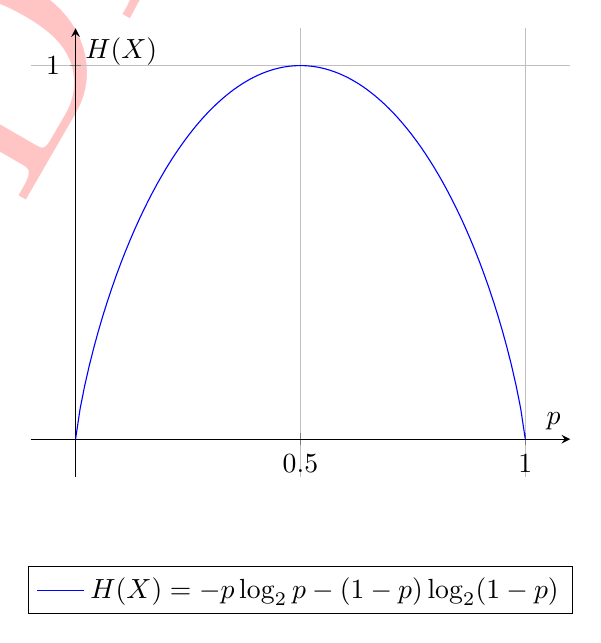
\begin{tikzpicture}
			\begin{axis}[
				xlabel={$p$},
				ylabel={$H(X)$},
				xmin=0, xmax=1,
				ymin=0, ymax=1,
				xtick={0,0.5,1},
				ytick={0,1},
				axis lines=middle,
				enlargelimits=true,
				clip=false,
				grid=major,
				legend style={at={(0.5,-0.2)},anchor=north},
				legend cell align=left,
				]
				\addplot[blue,domain=0:1,samples=100] {-x*log2(x)-(1-x)*log2(1-x)};
				\legend{$H(X)=-p\log_2 p-(1-p)\log_2(1-p)$}
			\end{axis}
		\end{tikzpicture}
		\caption{The entropy of a policy over two actions with $\pi(a|s) = p$}
	\end{figure}
\end{frame}


\subsection{Eligibility Traces}
\begin{frame}
	\frametitle{TD($\lambda$) using Eligibility Traces}
	
	\begin{block}{TD(0) update}
		$$
		\hat{V}_\pi(s_t)  \leftarrow
		\hat{V}_\pi(s_t) + \alpha \left( r_{t+1} + \gamma \hat{V}_\pi(s_{t+1}) - \hat{V}_\pi(s_t) \right) 
		$$
	\end{block}
	
	\begin{itemize}
		\item Only provides an update based on the most recent state
		\pause
		\item What if the pivotal action was taken far in the past,
		that lead to this desirable state?
		\pause
	\end{itemize}
	
	One solution is to keep track of the \textbf{Eligibility Trace}, the number of times a state has been visited, discounted
	geometrically via a parameter $\lambda$, called the \textbf{trace decay}, and by $\gamma$, the \textbf{discount rate}.
	\begin{align*}
		E^0(s) &:= 0 \\
		E^t(s) &:= \gamma \lambda E^{t-1}(s) + \delta_{s, s_t}
	\end{align*}
	
	\pause
	
			\textbf{Motivation:} States that are more recent/have bee
			
	The discounting allows for more recent visits to contribute more to the count than past visits (which may be valuable for
	non-stationary environments.)
	\pause
	
\end{frame}

\begin{frame}
	\frametitle{Generalised Advantage Estimation}
	
	Penalising TD updates using the eligibility trace, this gives us the update rule for TD($\lambda$). On timestep $t$, perform update
	\begin{align*}
		\forall s \in \mathcal{S}, \hat{V}_\pi(s) & := \hat{V}_\pi(s) + \alpha \red{E^t(s)}  \left( r_{t+1} + \gamma \hat{V}_\pi(s_{t+1}) - \hat{V}_\pi(s_t) \right)  \\
	\end{align*}
	Above expression can be unrolled for the advantage function (exercise to reader.) 
	$$
	\hat{A}_t = \delta_t +(\gamma \lambda)\delta_{t+1} + \ldots + 
	(\gamma \lambda)^{T-t+1} \delta_{T-1}
	$$
	where
	$\delta_t = r_t + \gamma V(s_{t+1}) - V(s_t)$.
\end{frame}



\begin{frame}
	\frametitle{References}
	
	\begin{itemize}
		\item Sutton and Barto, Reinforcement Learning: An Introduction \url{http://incompleteideas.net/book/the-book-2nd.html}
		\item OpenAI Intro to Policy Optimisation \url{https://spinningup.openai.com/en/latest/spinningup/rl_intro3.html}
		\item PPO Paper
		\url{https://arxiv.org/pdf/1707.06347.pdf}
		\item Generalised Advantage Estimation
		\url{https://arxiv.org/pdf/1506.02438.pdf}
		\item \bs
	\end{itemize}
\end{frame}

\begin{frame}
\frametitle{References}

\begin{itemize}
	\item Sutton and Barto, Reinforcement Learning: An Introduction \url{http://incompleteideas.net/book/the-book-2nd.html}
		\item Yan LeCun's cake analogy, NeurIPS 2016,\url{https://www.youtube.com/watch?v=Ount2Y4qxQo&t=1072s}
	\item Jay Bailey's DQN Distillation \url{https://www.lesswrong.com/posts/kyvCNgx9oAwJCuevo/deep-q-networks-explained}
	\item Playing Atari with Deep Reinforcement Learning
	\url{https://www.cs.toronto.edu/~vmnih/docs/dqn.pdf}
	\item Human-level control through deep reinforcement learning
	\url{https://www.nature.com/articles/nature14236}
	\item Rainbow DQN \url{https://arxiv.org/abs/1710.02298}
\end{itemize}
\end{frame}



\begin{frame}
\frametitle{Robins-Monro Convergence conditions}

The Robins-Monro convergence conditions are properties of the learning rate that
are usually required in most proofs to ensure convergence.

Let $\alpha_t$ denote the learning rate at time $t$. Then the conditions are

$$
\sum_{t=1}^\infty \alpha_t = \infty \text{ and } \sum_{t=1}^\infty \alpha_t^2 < \infty
$$

Intuitively, the first condition ensures that the steps are large enough to eventually overcome
any initial conditions/random fluctuations, and the second condition ensures that eventually the 
steps become small enough to ensure convergence.
\pause 

An example of such a learning rate would be $\alpha_t = 1/t$.

Note that the usual method of choosing $\forall t, \alpha_t = \alpha \in \mathbb{R}$ 
fails the RM conditions.
\end{frame}



\end{document}